\documentclass[journal,twoside,web]{ieeecolor}
\usepackage{generic}
\usepackage{cite}
\usepackage{amsmath,amssymb,amsfonts}
\usepackage{algorithmic}
\usepackage{graphicx}
\usepackage{tikz}
\usetikzlibrary{arrows.meta,positioning}
\usepackage{booktabs}
\usepackage{algorithm,algorithmic}
\usepackage{hyperref}
\hypersetup{hidelinks}
\usepackage{textcomp}
\def\BibTeX{{\rm B\kern-.05em{\sc i\kern-.025em b}\kern-.08em
    T\kern-.1667em\lower.7ex\hbox{E}\kern-.125emX}}
\markboth{\hskip25pc IEEE TRANSACTIONS AND JOURNALS TEMPLATE}
{Author \MakeLowercase{\textit{et al.}}: Title}
\begin{document}
\title{Few-Shot Continual Learning for 3D Brain MRI with Frozen Foundation Models}

% ---------------------------------------------------------------------------
% REVISION NOTE (2026-09-12). All numbers in this file come from the corrected
% protocol (PROTOCOL_AUDIT.md): subject-grouped held-out test set, whole-volume
% sliding-window inference (overlap 0.25), per-case metrics, real IXI ages,
% unlabelled BraTS cases excluded. Values are mean +/- SD over seeds 42-44 from
% outputs/benchmark_v2/n32/. The pre-audit manuscript is preserved as
% main_v1_original_2026-09-05.tex.
% ---------------------------------------------------------------------------

\author{Chi-Sheng Chen$^{1}$,
Xinyu Zhang$^{2}$,
En-Jui Kuo$^{5}$,
Rong Fu$^{2}$,
Qiuzhe Xie$^{3}$,
and Fan Zhang$^{4}$
\thanks{$^{1}$Beth Israel Deaconess Medical Center \& Harvard Medical School, Boston, MA 02115 USA.}
\thanks{$^{2}$Luddy School of Informatics, Computing, and Engineering, Indiana University Bloomington, Bloomington, IN 47405 USA.}
\thanks{$^{3}$Institute of Electronics Engineering, National Taiwan University, 106319, Taiwan.}
\thanks{$^{4}$Department of Mathematics, Boise State University, Boise, ID 83702 USA.}
\thanks{$^{5}$Department of Electrophysics, National Yang Ming Chiao Tung University, 30010, Taiwan.}}

\maketitle

\begin{abstract}
Foundation models pretrained on large 3D medical imaging corpora must often be adapted to a sequence of downstream tasks from few labeled examples, without revisiting earlier tasks' data. We study this few-shot continual setting on 3D brain MRI with a frozen FOMO pretrained 3D U-Net, adapting it to glioma segmentation (BraTS 2023) and then brain-age regression (IXI) from 32 labeled volumes per task. Each task receives its own Low-Rank Adaptation (LoRA) module and output head, so earlier tasks are never modified. Under a subject-grouped held-out protocol with whole-volume inference and three seeds, we find that most of the segmentation deficit previously attributed to LoRA is a configuration artefact: leaving the 66-parameter segmentation output projection frozen costs 0.22 Dice (paired $p<10^{-130}$ over 820 test cases). With that projection trainable and rank 16, LoRA reaches Dice $0.777\pm0.004$, trailing linear probing of the full decoder ($0.789\pm0.005$) by 0.012 Dice (1.5\% relative; paired $p=3{\times}10^{-10}$) while training 90$\times$ fewer parameters (0.41\% vs.\ 37.4\% of the network) with the same seed-to-seed stability, and trailing full fine-tuning ($0.798\pm0.025$) by 0.021 Dice; full fine-tuning in turn forgets $0.33\pm0.06$ Dice on the first task after learning the second, and 0.41 Dice when a third task of the same type---ISLES 2022 stroke-lesion segmentation---is inserted between them, while the frozen methods forget nothing across all three. We also report a negative result: at 32 shots, no method---including full fine-tuning of all 22.6M parameters---learns brain age from $64^3$ patches, all landing at MAE 14.4--14.6\,yr against a constant-predictor baseline of 14.6\,yr. Together these results position adapter isolation as a parameter-cost trade-off rather than a forgetting argument, since frozen-encoder linear probing is likewise forgetting-free at higher accuracy, and they document an evaluation protocol whose absence had previously inflated every number in this setting.
\end{abstract}

\begin{IEEEkeywords}
Few-shot learning \and Continual learning \and LoRA \and 3D brain MRI \and Foundation models \and Parameter-efficient fine-tuning.
\end{IEEEkeywords}

\section{Introduction}
\label{sec:introduction}

\IEEEPARstart{M}{edical} imaging AI increasingly relies on foundation models pretrained on large-scale datasets~\cite{fomo2025,baseline}. \label{sec:intro}
When deployed in clinical settings, these models must adapt to multiple tasks---e.g., tumor segmentation and brain age estimation---often with limited labeled data and without access to prior task samples due to privacy or storage constraints. In practice, radiology departments may introduce new analysis tasks over time (e.g., adding brain age prediction to an existing tumor workflow) with only a small batch of newly annotated cases. This scenario motivates \emph{few-shot continual learning}: learning new tasks sequentially from few examples while retaining performance on previously learned tasks.

Sequential fine-tuning of shared backbone parameters typically causes \emph{catastrophic forgetting}~\cite{kirkpatrick2017,mccloskey1989catastrophic}: when the model is updated for a new task, performance on prior tasks degrades. Regularization- and distillation-based remedies such as EWC~\cite{kirkpatrick2017} and LwF~\cite{li2017lwf} soften this at the cost of tuning effort and only approximate protection. An alternative is to \emph{freeze} the pretrained backbone and adapt only small task-specific modules. Parameter-efficient fine-tuning methods such as LoRA~\cite{hu2022lora, hu2024computational} inject low-rank matrices into selected layers, training a small fraction of parameters while preserving the original weights.

We study a frozen FOMO-style pretrained 3D U-Net~\cite{fomo2025} adapted with task-specific LoRA modules to two heterogeneous tasks in sequence---glioma segmentation on BraTS 2023 and brain-age regression on IXI---from 32 labeled volumes each. The premise is simple: because the backbone and prior adapters are never modified, earlier tasks cannot be forgotten. The interesting questions are what this costs in accuracy relative to training more of the network, and whether the frozen backbone is adequate for both task types.

Answering those questions required first fixing how they are measured. In the course of this work we found that the evaluation pipeline commonly used for this setting---and used in an earlier version of this manuscript---reports on the split used for model selection, scores a single random $64^3$ crop per case, pools voxels across cases into one Dice, and lets longitudinal timepoints of one patient span train and test. We replaced it with subject-grouped train/validation/test splits, whole-volume sliding-window inference, and per-case Dice and 95th-percentile Hausdorff distance (HD95). Every number below is from that protocol.

Our findings and contributions are:
\begin{itemize}
\item \textbf{Most of the LoRA segmentation gap is a configuration artefact.} Applying LoRA to encoder and decoder while leaving the segmentation output projection---66 parameters---at its pretrained value yields Dice $0.538\pm0.082$. Making those 66 parameters trainable yields $0.754\pm0.029$, a paired gain of $+0.217$ ($p<10^{-130}$, $n=820$ cases over three seeds) at unchanged parameter budget.
\item \textbf{At rank 16, LoRA trades 0.012 Dice for a 90$\times$ smaller trainable budget.} LoRA with a trainable output head trails frozen-encoder linear probing of the full decoder by $0.012$ Dice (paired 95\% CI $[0.008, 0.015]$; $-0.013$, $-0.013$, $-0.009$ on the three seeds) while training 93.8K rather than 8.45M parameters, matches its seed stability (SD 0.004 vs.\ 0.005), and trails full fine-tuning by $0.021$ Dice; full fine-tuning forgets $0.33$ Dice on segmentation after learning regression. Rank 8, the usual default, leaves three times that gap and seven times the variance.
\item \textbf{Same-type tasks forget the most.} In a three-task sequence---BraTS glioma, then ISLES stroke-lesion segmentation, then brain age---full fine-tuning drops BraTS Dice from 0.798 to 0.385 after learning ISLES and loses 0.20 on ISLES after brain age; it is also the least accurate method on ISLES itself (0.387 vs.\ 0.41--0.42 for the frozen methods). Adapter isolation and frozen-encoder linear probing forget nothing at any step.
\item \textbf{Zero forgetting is not a differentiator.} Frozen-encoder linear probing also has backward transfer exactly zero, because nothing shared is updated, and it is the more accurate of the two forgetting-free methods. The case for adapter isolation is therefore parameter and storage cost, not forgetting or accuracy.
\item \textbf{A negative result on brain age.} At 32 shots with $64^3$ patch input, no method---LoRA, linear probing, or full fine-tuning---beats the constant predictor (MAE 14.4--14.6\,yr; $R^2\approx 0$; prediction standard deviation $\le 1.4$\,yr on average against a true spread of 16.5\,yr). We report this rather than the near-zero errors an earlier pipeline produced against placeholder labels.
\item \textbf{A corrected evaluation protocol and code}, with tests that guard the label-handling and split-leakage failures we encountered.
\end{itemize}


\section{Related Work}
\label{sec:related}

\subsection{Foundation Models for Medical Imaging}

Large-scale pretrained models have transformed medical image analysis. The FOMO initiative~\cite{fomo2025} provides 3D foundation models pretrained on diverse medical imaging datasets via masked autoencoding objectives, yielding general-purpose representations for downstream adaptation. UNETR~\cite{unetr} introduced Vision Transformers into 3D medical segmentation by replacing CNN encoders with self-attention, demonstrating strong performance on multi-organ and brain tumor segmentation. More recently, SAM-Med3D~\cite{sammed3d} extended the Segment Anything paradigm to volumetric data, and domain-specific foundation models have emerged for pathology~\cite{chen2024towards} and radiology. These models share a common deployment challenge: adapting to multiple downstream tasks efficiently while preserving the pretrained representations, particularly when labeled data is scarce.

\subsection{Continual Learning in Medical Imaging}

Continual learning addresses the problem of sequentially learning new tasks without forgetting previously acquired knowledge~\cite{mccloskey1989catastrophic}. Classical approaches fall into three categories: (i)~\emph{regularization-based} methods such as EWC~\cite{kirkpatrick2017} and Synaptic Intelligence~\cite{zenke2017continual}, which penalize changes to important parameters; (ii)~\emph{replay-based} methods such as iCaRL~\cite{rebuffi2017icarl}, which store or generate exemplars from prior tasks; and (iii)~\emph{distillation-based} methods such as LwF~\cite{li2017lwf}, which use the previous model's outputs as soft targets. In medical imaging, continual learning has been explored primarily for class-incremental segmentation: LifeLonger~\cite{derakhshani2022lifelonger} benchmarks continual disease classification across dermatology datasets, while Lifelong nnU-Net~\cite{gonzalez2023lifelong} standardizes continual organ segmentation. However, most prior work considers \emph{class-incremental} settings with homogeneous outputs (e.g., adding new organ classes). Our work addresses \emph{task-incremental} continual learning across \emph{heterogeneous} output types---segmentation and regression---which presents distinct challenges since the task heads and loss functions differ fundamentally.

\subsection{Parameter-Efficient Fine-Tuning}

Parameter-efficient fine-tuning (PEFT) methods adapt large pretrained models by training only a small subset of parameters. LoRA~\cite{hu2022lora} injects trainable low-rank decompositions into weight matrices, achieving competitive performance with full fine-tuning at a fraction of the parameter cost. Alternative PEFT approaches include Adapters~\cite{houlsby2019}, which insert bottleneck modules between layers; Prefix-Tuning~\cite{prefix_tuning}, which prepends learnable tokens to the input; and BitFit~\cite{bitfit}, which tunes only bias terms. In the context of continual learning, PEFT methods offer a natural mechanism for task isolation: PackNet~\cite{packnet} iteratively prunes and freezes network capacity per task, while Piggyback~\cite{piggyback} learns binary masks over a shared backbone. Our approach is most closely related to adapter-isolation strategies but applies LoRA's low-rank structure to 3D convolutions, which is directly compatible with pretrained U-Net architectures. A recurring detail in the PEFT literature, and the one that turns out to matter most here, is that the task-specific output layer is always trained alongside the low-rank updates; a pretrained projection cannot be expected to map onto a new label space.


\section{Method}
\label{sec:method}

\subsection{Problem Formulation}
\label{sec:problem}

We consider continual learning with sequential task arrival. Let $f_\theta$ denote a pretrained 3D U-Net backbone (frozen) and $\mathcal{T}_1, \mathcal{T}_2, \ldots, \mathcal{T}_K$ a sequence of tasks. For each task $k$, we have access to only $N_k$ labeled few-shot samples ($N_k = 32$ throughout) drawn from task-specific distribution $\mathcal{D}_k = \{(x_i^{(k)}, y_i^{(k)})\}_{i=1}^{N_k}$. We assume \emph{no replay}: when training on $\mathcal{T}_k$, we cannot access data from $\mathcal{T}_{<k}$. The optimization objective for task $k$ is:
\begin{equation}
\min_{\phi_k, h_k} \; \frac{1}{N_k} \sum_{i=1}^{N_k} \mathcal{L}_k \bigl( h_k(f_\theta(x_i^{(k)}; \phi_k)),\; y_i^{(k)} \bigr)
\label{eq:objective}
\end{equation}
where $\phi_k$ denotes the LoRA adapter parameters for task $k$, $h_k$ the task-specific head, and $\mathcal{L}_k$ the task loss. Crucially, $\theta$ remains frozen throughout; only $\phi_k$ and $h_k$ are optimized. The goal is to learn $\{\phi_k, h_k\}_{k=1}^K$ such that performance on all seen tasks remains high after training on $\mathcal{T}_K$.

We evaluate two tasks: (1) tumor segmentation (3D binary mask) and (2) brain age estimation (regression). Each task has modality-specific inputs (BraTS: T2w, T2-FLAIR, T1c; IXI: T1, T2) and a distinct output head $h_k$. Because the modality counts differ, the first convolution of the encoder cannot be shared and is task-specific; all remaining encoder weights (39 of 40 tensors) are shared and frozen.

Figure~\ref{fig:framework} illustrates the overall pipeline: a frozen pretrained backbone, task-specific LoRA adapters, and task heads. At inference for task $k$, we use backbone $f_\theta$ + adapter $\phi_k$ + head $h_k$; prior adapters and the backbone remain frozen. Task identity is assumed known at inference.

\begin{figure*}[t]
\centering
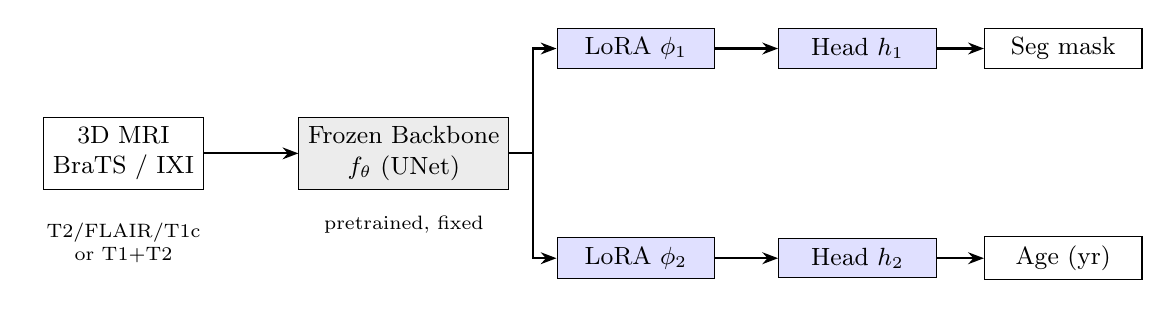
\begin{tikzpicture}[
  node distance=0.5cm and 0.8cm,
  box/.style={draw, minimum width=2cm, minimum height=0.5cm, align=center, font=\small},
  bigbox/.style={draw, minimum width=2.2cm, minimum height=0.7cm, align=center, font=\small},
  frozen/.style={fill=gray!15, box},
  trainable/.style={fill=blue!12, box},
  arrow/.style={-{Stealth[length=2mm]}, thick}
]
  \node[box] (input) {3D MRI\\BraTS / IXI};
  \node[below=0.3cm of input, font=\scriptsize, text width=2.2cm, align=center] {T2/FLAIR/T1c or T1+T2};
  \node[bigbox, frozen, right=1.2cm of input] (backbone) {Frozen Backbone\\$f_\theta$ (UNet)};
  \node[below=0.2cm of backbone, font=\scriptsize] {pretrained, fixed};
  \node[box, trainable, above right=0.6cm and 0.6cm of backbone] (lora1) {LoRA $\phi_1$};
  \node[box, trainable, below right=0.6cm and 0.6cm of backbone] (lora2) {LoRA $\phi_2$};
  \node[box, trainable, right=0.8cm of lora1] (head1) {Head $h_1$};
  \node[box, trainable, right=0.8cm of lora2] (head2) {Head $h_2$};
  \node[box, right=0.6cm of head1] (out1) {Seg mask};
  \node[box, right=0.6cm of head2] (out2) {Age (yr)};
  \draw[arrow] (input) -- (backbone);
  \draw[arrow] (backbone.east) -- ++(0.3,0) |- (lora1.west);
  \draw[arrow] (backbone.east) -- ++(0.3,0) |- (lora2.west);
  \draw[arrow] (lora1) -- (head1);
  \draw[arrow] (lora2) -- (head2);
  \draw[arrow] (head1) -- (out1);
  \draw[arrow] (head2) -- (out2);
\end{tikzpicture}
\caption{Framework: frozen pretrained backbone $f_\theta$ with task-specific LoRA adapters $\phi_k$ and heads $h_k$. Gray = frozen; blue = trainable per task. At inference for T1 (resp.\ T2): backbone + $\phi_1$ + $h_1$ (resp.\ $\phi_2$ + $h_2$). For segmentation, $h_1$ is the $1{\times}1{\times}1$ output projection of the U-Net decoder (66 parameters); leaving it frozen is the single largest source of error we observed (Sec.~\ref{sec:res_head}).}
\label{fig:framework}
\end{figure*}

\subsection{LoRA for 3D Convolutions}
\label{sec:lora}

Low-Rank Adaptation (LoRA)~\cite{hu2022lora} injects trainable low-rank matrices into a frozen weight matrix $W \in \mathbb{R}^{d \times k}$:
\begin{equation}
W' = W + \Delta W, \quad \Delta W = \frac{\alpha}{r} B \cdot A, \quad A \in \mathbb{R}^{r \times k}, \; B \in \mathbb{R}^{d \times r}
\label{eq:lora}
\end{equation}
with rank $r \ll \min(d,k)$ and scaling factor $\alpha$. Only $A$ and $B$ are trained; $W$ stays frozen. The scaling ratio $\alpha/r$ controls the magnitude of the low-rank perturbation relative to the pretrained weights.

For 3D convolutions in a U-Net, we apply LoRA via parallel $1\times1\times1$ convolutions acting on the channel dimension:
\begin{equation}
\text{Conv3d}'(x) = \text{Conv3d}(x; W) + \frac{\alpha}{r} \, \text{Conv1}(x; B) \circ \text{Conv1}(x; A)
\label{eq:lora3d}
\end{equation}
where Conv1 denotes $1\times1\times1$ convolution, $A \in \mathbb{R}^{r \times C_{\text{in}}}$ projects to rank-$r$ space, and $B \in \mathbb{R}^{C_{\text{out}} \times r}$ projects back. This formulation is memory-efficient and compatible with standard Conv3d layers~\cite{peft}.

We use $\alpha=16$, evaluate $r \in \{4, 8, 16\}$ (Sec.~\ref{sec:res_rank}) and report $r=16$, and target every Conv3d in both encoder and decoder for segmentation; encoder-only suffices for regression. For a single Conv3d layer with input channels $C_{\text{in}}$ and output channels $C_{\text{out}}$, the number of LoRA parameters is:
\begin{equation}
|\phi_{\text{layer}}| = r \cdot (C_{\text{in}} + C_{\text{out}})
\label{eq:param_count}
\end{equation}
which is substantially smaller than the original $C_{\text{out}} \times C_{\text{in}} \times D \times H \times W$ parameters. Summed over all targeted layers at $r=16$, the adapter for segmentation has 93,810 parameters against a 22.63M-parameter U-Net (0.41\%), and the adapter for regression has 55,841 parameters against the 14.16M-parameter encoder-plus-head (0.39\%); at $r=8$ the counts are 46,872 and 28,177.

\subsection{Continual Learning via Adapter Isolation}
\label{sec:continual}

Each task $k$ receives a \emph{dedicated LoRA adapter} $\phi_k$. The full training and inference procedure is summarized in Algorithm~\ref{alg:continual}. The trainable parameter set for task $k$ is strictly disjoint from all other tasks:
\begin{equation}
\Phi_k = \{\phi_k, h_k\}, \quad \Phi_i \cap \Phi_j = \emptyset \;\; \forall \, i \neq j
\label{eq:disjoint}
\end{equation}
Because $\theta$ and $\{\Phi_{<k}\}$ are frozen when optimizing $\Phi_k$, the performance of any prior task $j < k$ is invariant to training on $\mathcal{T}_k$. Formally, let $R_{t,j}$ denote the performance of task $j$ after training up to task $t$. Then:
\begin{equation}
R_{t,j} = R_{j,j} \quad \forall \, t \geq j \implies \text{BWT}_j = R_{K,j} - R_{j,j} = 0
\label{eq:bwt_zero}
\end{equation}
This zero-forgetting property holds \emph{by construction}, without regularization or replay. It is not, however, unique to adapters: any scheme that leaves shared weights untouched---including linear probing on a frozen encoder---satisfies Eq.~\eqref{eq:bwt_zero} equally. What distinguishes the schemes is how many parameters they must train to reach a given accuracy, which is what Section~\ref{sec:results} measures. The total model storage after $K$ tasks is:
\begin{equation}
\text{Storage} = |\theta| + \sum_{k=1}^{K} (|\phi_k| + |h_k|)
\label{eq:storage}
\end{equation}
which grows linearly in $K$ with a small per-task overhead since $|\phi_k| \ll |\theta|$.

\begin{algorithm}[t]
\caption{Continual Learning via LoRA Adapter Isolation}
\label{alg:continual}
\begin{algorithmic}[1]
\REQUIRE Pretrained backbone $f_\theta$; task sequence $\mathcal{T}_1, \ldots, \mathcal{T}_K$; subject-grouped train/val/test splits per task; LoRA rank $r$; epochs $E$
\ENSURE Trained adapters $\{\phi_k\}_{k=1}^K$ and heads $\{h_k\}_{k=1}^K$
\STATE Freeze all parameters of $f_\theta$
\FOR{$k = 1$ \TO $K$}
    \STATE Initialize LoRA adapter $\phi_k$ with rank $r$ (Kaiming $A$, zero $B$)
    \STATE Initialize task head $h_k$ (output projection for segmentation; pooled regressor for regression); mark trainable
    \IF{$k > 1$}
        \STATE Freeze all previous adapters $\phi_1, \ldots, \phi_{k-1}$ and heads $h_1, \ldots, h_{k-1}$
    \ENDIF
    \FOR{epoch $= 1$ \TO $E$}
        \FOR{each mini-batch $(x, y) \in \mathcal{D}_k^{\text{train}}$}
            \STATE $\hat{y} \leftarrow h_k(f_\theta(x; \phi_k))$
            \STATE Update $\phi_k, h_k$ on $\mathcal{L}_k(\hat{y}, y)$ with AdamW
        \ENDFOR
        \STATE Score $\mathcal{D}_k^{\text{val}}$ (deterministic centre crop); keep the best epoch
    \ENDFOR
    \STATE Score the kept checkpoint once on $\mathcal{D}_k^{\text{test}}$ with whole-volume inference
\ENDFOR
\end{algorithmic}
\end{algorithm}

\subsection{Task Heads and Losses}
\label{sec:heads}

\textbf{Task 1 (Segmentation).} The full U-Net decoder produces a voxel-wise two-class prediction. LoRA is applied to every Conv3d in encoder and decoder. The head $h_1$ is the decoder's final $1{\times}1{\times}1$ projection from 32 channels to the 2 output classes (66 parameters), which is trained from its pretrained initialization. We stress this because a natural but wrong reading of ``frozen backbone'' is to freeze this layer too; Section~\ref{sec:res_head} quantifies the consequence. The training loss is cross-entropy plus soft Dice on the foreground probability:
\begin{equation}
\mathcal{L}_{\text{seg}} = \text{CE}(p, g) + 1 - \frac{2 \sum_i p_i g_i + \epsilon}{\sum_i p_i + \sum_i g_i + \epsilon}
\end{equation}
where $p_i$ is the softmax foreground probability at voxel $i$, $g_i$ the binary label, and $\epsilon=10^{-8}$.

\textbf{Task 2 (Regression).} For brain age estimation we use the encoder only: its deepest feature map is global-average-pooled and passed through a two-layer fully connected head with a single scalar output. LoRA targets the encoder's Conv3d layers. The loss is mean squared error in years.

\textbf{Optimization.} All methods use AdamW (learning rate $10^{-3}$, weight decay $10^{-5}$) with cosine annealing to $10^{-6}$ over 100 epochs, batch size 2, gradient-norm clipping at 1.0, and LoRA dropout 0.1. Training patches are random $64^3$ crops; no other augmentation is used. Hyperparameters are identical across methods and were not tuned per method.

\section{Experiments}
\label{sec:experiments}

\subsection{Datasets}
\label{sec:data}

\textbf{Notation.} T1 denotes tumor segmentation, T2 brain-age regression, and T3 stroke-lesion segmentation. The main comparison uses the sequence T1$\to$T2; Section~\ref{sec:res_three} inserts T3 between them (T1$\to$T3$\to$T2).

\textbf{T1: BraTS 2023 Glioma}~\cite{brats2023}. We use the 1251 labeled volumes of the training release, with channels T2w, T2-FLAIR and T1c and a binary whole-tumor mask derived from the expert annotation. The challenge's validation release ships without segmentations and is excluded; an earlier pipeline had written those 219 volumes with all-zero masks, which are indistinguishable from a tumor-free label and had contaminated 17\% of the test set. Several subjects contribute more than one longitudinal timepoint; these are kept in the same split.

\textbf{T2: IXI}~\cite{ixi}. Of the 577 subjects with both T1 and T2 scans, 559 have a usable age in the IXI demographics table (15 have no table entry, 3 have a missing age) and are used; none is imputed. Test-set ages span 20.0--86.3\,yr (mean 50.0, SD 16.5).

\textbf{T3: ISLES 2022.} Ischemic-stroke lesion segmentation with channels DWI, ADC and FLAIR (FLAIR resampled onto the DWI grid) and the expert lesion mask; 247 of the 250 cases are used, three being excluded because their mask emptied under 1\,mm resampling. Lesions are small (median $\approx$775 voxels), which makes this a harder segmentation task than T1 and one drawn from a single cohort, so unlike an earlier infarct-\emph{classification} design that contrasted ISLES with IXI controls, it carries no acquisition confound.

\textbf{Data use.} BraTS 2023 was obtained from Synapse (syn51156910) under its Data Use Agreement; IXI is publicly available at \url{https://brain-development.org/ixi-dataset/}; ISLES 2022 is distributed under CC BY 4.0 (Zenodo 7153326). No additional ethics approval was required.

\textbf{Preprocessing.} Volumes are resampled to 1\,mm isotropic and z-scored per channel over non-zero voxels.

\subsection{Splits and Evaluation Protocol}
\label{sec:protocol}

For each task and seed we draw a subject-grouped three-way split: a training set of exactly $N_k=32$ volumes, a validation set of 60 subjects used only for epoch selection, and a held-out test set of up to 250 subjects (275 volumes for T1, 250 for T2, all 155 remaining subjects for T3) on which every number in this paper is reported. No subject appears in more than one split. Splits are persisted so that all methods are scored on identical cases, which is what makes the paired comparisons below valid.

\textbf{Segmentation} is scored on the whole volume by Gaussian-weighted sliding-window inference ($64^3$ windows, 25\% overlap), followed by argmax. We report per-case Dice and per-case HD95 in voxel units, averaged over cases. \textbf{Regression} is scored by averaging the prediction over a fixed $2{\times}2{\times}2$ grid of $64^3$ windows. We report MAE in years, $R^2$, and the standard deviation of the predictions, the last because it exposes a model that has collapsed to a constant regardless of MAE.

\textbf{Backward transfer.} For the sequential baselines, after each later task we re-score every earlier task's test set with that task's own head on the now-updated encoder and report $\text{BWT}_j = R_{K,j} - R_{j,j}$ in Dice; in the three-task sequence we also report the intermediate value after T3. For adapter-isolated methods this quantity is zero by construction and is not re-measured.

\subsection{Backbone}
\label{sec:backbone}

\texttt{unet\_b} from FOMO~\cite{fomo2025}, initialized from \texttt{fomo25\_mmunetvae\_pretrained.ckpt}. All 40 encoder tensors except the modality-specific input convolution load from the checkpoint; the decoder loads 59 of 82 tensors, the remainder being normalization parameters. The same checkpoint is loaded at the start of every task for every method.

\subsection{Compared Methods}
\label{sec:baselines}

All methods share the backbone, data, splits, optimizer and schedule; they differ only in which parameters are trainable (Table~\ref{tab:params}).
\begin{itemize}
\item \textbf{LoRA (enc+dec).} Rank-8 LoRA on every Conv3d; output projection frozen. This is the configuration of the earlier version of this work.
\item \textbf{LoRA + head (proposed).} As above, plus the 66-parameter output projection. Reported at rank 16; ranks 4 and 8 appear in the ablation of Sec.~\ref{sec:res_rank}.
\item \textbf{Sequential Linear.} Encoder frozen; every downstream parameter trainable. For segmentation this is the entire decoder (8.45M parameters); for regression, the 513-parameter head. One model carried through the sequence.
\item \textbf{Sequential FT.} All parameters trainable; one model carried through the sequence. The forgetting reference.
\end{itemize}
Regularization- and replay-based baselines (EWC, LwF, experience replay) and the per-task oracles that appeared in an earlier version were run under the pre-audit protocol only and are omitted here rather than reported on a different footing.

\begin{table}[t]
\caption{Trainable parameters per method. The comparison in Table~\ref{tab:main} spans four orders of magnitude of trainable budget.}
\label{tab:params}
\centering
\footnotesize
\setlength{\tabcolsep}{4pt}
\begin{tabular}{lrrrr}
\toprule
 & \multicolumn{2}{c}{T1 segmentation} & \multicolumn{2}{c}{T2 regression} \\
\cmidrule(lr){2-3} \cmidrule(lr){4-5}
Method & trainable & share & trainable & share \\
\midrule
LoRA (enc+dec), $r{=}8$   & 46,872     & 0.207\%  & 28,177     & 0.199\% \\
LoRA + head, $r{=}8$      & 46,938     & 0.207\%  & 28,177     & 0.199\% \\
LoRA + head, $r{=}16$     & 93,810     & 0.414\%  & 55,841     & 0.393\% \\
Sequential Linear         & 8,446,306  & 37.4\%   & 513        & 0.004\% \\
Sequential FT             & 22,582,978 & 100\%    & 14,136,321 & 100\% \\
\bottomrule
\end{tabular}
\end{table}

\subsection{Implementation and Resources}
\label{sec:impl}

Experiments run on a single NVIDIA RTX 3090. Measured peak GPU memory is 1.67\,GB during segmentation training (batch 2) and 4.16\,GB during whole-volume evaluation (batch 8 windows); regression peaks at 0.69\,GB and 2.53\,GB respectively. One segmentation run trains in 46\,min and evaluates 275 volumes in about 25\,min; regression trains in 14\,min. Code, splits and per-case predictions are released with the paper.

\section{Results}
\label{sec:results}

All results are on the held-out test split at $N_k=32$, reported as mean $\pm$ SD over three seeds (42--44); each seed draws its own subject-grouped split, and all methods share the split within a seed. Paired comparisons pool the per-case differences across seeds ($n = 3 \times 275 = 820$ for T1).

\subsection{Main Comparison}
\label{sec:main}

\begin{table*}[t]
\caption{Held-out test results, $N_k=32$, mean $\pm$ SD over seeds 42--44. T1 = BraTS glioma segmentation (275 volumes, 250 subjects per seed); T2 = IXI brain age (250 subjects per seed). ``T1 after T2'' is T1 re-scored after the model has learned T2; BWT is its change. Constant-predictor MAE for T2 is $\approx$14.6\,yr. Pred.\ SD is the standard deviation of the predicted ages (true SD 16.5).}
\label{tab:main}
\centering
\footnotesize
\setlength{\tabcolsep}{3.5pt}
\begin{tabular}{lcccccccc}
\toprule
 & \multicolumn{2}{c}{T1 segmentation} & \multicolumn{3}{c}{T2 brain age} & \multicolumn{2}{c}{Forgetting} & \\
\cmidrule(lr){2-3} \cmidrule(lr){4-6} \cmidrule(lr){7-8}
Method & Dice$\uparrow$ & HD95$\downarrow$ & MAE (yr)$\downarrow$ & $R^2$ & pred.\ SD & T1 after T2 & BWT & Trainable \\
\midrule
LoRA (enc+dec), $r{=}8$   & $0.538\pm0.082$ & $135.1\pm14.0$ & $14.51\pm0.39$ & $-0.06\pm0.06$ & 1.40 & = T1 & 0.000 & 0.21\% \\
LoRA + head, $r{=}16$     & $0.777\pm0.004$ & $43.2\pm0.7$   & $14.72\pm0.37$ & $-0.09\pm0.05$ & 1.06 & = T1 & 0.000 & \textbf{0.41\%} \\
Sequential Linear  & $0.789\pm0.005$ & $41.9\pm1.3$   & $14.64\pm0.12$ & $-0.06\pm0.03$ & 0.57 & $0.789\pm0.005$ & 0.000 & 37.4\% \\
Sequential FT      & $\mathbf{0.798\pm0.025}$ & $\mathbf{40.2\pm4.9}$ & $14.52\pm0.10$ & $-0.03\pm0.03$ & 0.62 & $0.470\pm0.084$ & $-0.328\pm0.062$ & 100\% \\
\bottomrule
\end{tabular}
\end{table*}

\begin{table}[t]
\caption{Paired differences in per-case T1 Dice, pooled over the three seeds ($n=820$ case-pairs; bootstrap 95\% CI; Wilcoxon signed-rank). L+h$_{r}$ = LoRA + head at rank $r$; SL = Sequential Linear; FT = Sequential FT; L$_8$ = LoRA (enc+dec), $r{=}8$. Per-seed L+h$_{16}-$SL: $-0.013$, $-0.013$, $-0.009$; per-seed L+h$_{8}-$SL: $-0.002$ ($p=0.28$), $-0.061$, $-0.043$.}
\label{tab:paired}
\centering
\footnotesize
\setlength{\tabcolsep}{4pt}
\begin{tabular}{lccc}
\toprule
Contrast & $\Delta$Dice & 95\% CI & $p$ \\
\midrule
L+h$_{16}$ $-$ SL         & $-0.012$ & $[-0.015,\,-0.008]$ & $3{\times}10^{-10}$ \\
FT $-$ L+h$_{16}$         & $+0.021$ & $[+0.017,\,+0.025]$ & $1{\times}10^{-33}$ \\
L+h$_{16}$ $-$ L+h$_{8}$  & $+0.024$ & $[+0.020,\,+0.027]$ & $5{\times}10^{-40}$ \\
L+h$_{8}$ $-$ SL          & $-0.035$ & $[-0.040,\,-0.030]$ & $9{\times}10^{-50}$ \\
L+h$_{8}$ $-$ L$_{8}$     & $+0.217$ & $[+0.207,\,+0.228]$ & $1{\times}10^{-134}$ \\
\bottomrule
\end{tabular}
\end{table}

Table~\ref{tab:main} gives the main comparison and Table~\ref{tab:paired} the paired tests. Three results carry the paper.

\subsection{The Output Projection Accounts for the LoRA Segmentation Gap}
\label{sec:res_head}

At rank 8, with the decoder's final $1{\times}1{\times}1$ projection frozen, LoRA on every other layer reaches Dice $0.538\pm0.082$ and HD95 $135\pm14$; the wide spread (0.452--0.648 across seeds) reflects how much the outcome depends on whether the pretrained projection happens to be usable for the new label. Training those 66 additional parameters lifts it to Dice $0.754\pm0.029$ and HD95 $48.6\pm5.0$---a paired gain of $+0.217$ Dice ($p = 1{\times}10^{-134}$) at a parameter budget that changes from 46,872 to 46,938, and a threefold reduction in seed variance. Mechanically this is unsurprising: the pretrained projection maps decoder channels onto the pretraining objective's output space, and rank-8 perturbations upstream cannot re-map it onto a new label space. Practically it matters because the frozen-projection configuration is the one an earlier version of this work reported; most, though not all, of the deficit it attributed to LoRA was this layer.

\subsection{Accuracy per Trainable Parameter}
\label{sec:res_cost}

Sequential Linear remains more accurate than LoRA + head at rank 16, but narrowly: Dice $0.789\pm0.005$ vs.\ $0.777\pm0.004$, a paired difference of $-0.012$ (95\% CI $[-0.015, -0.008]$, $p = 3{\times}10^{-10}$), and HD95 41.9 vs.\ 43.2; the two are equally stable across seeds. Sequential Linear reaches that accuracy by training the full 8.45M-parameter decoder; LoRA + head trains 93.8K, a factor of 90 fewer, for a 1.5\% relative Dice cost. Full fine-tuning of all 22.6M parameters is better still, by $+0.021$ Dice over LoRA + head ($p = 1{\times}10^{-33}$) and $+0.009$ over Sequential Linear, so the frozen backbone leaves some accuracy on the table for every frozen method---at a cost discussed next.

\subsection{Rank}
\label{sec:res_rank}

Table~\ref{tab:rank} varies the LoRA rank with the output head trainable. Rank 4 is not worse than rank 8 (paired $+0.007$, $p = 9{\times}10^{-6}$) at half the parameters, so rank 8 sits in a flat region; rank 16 is where the added capacity pays, gaining $+0.024$ Dice over rank 8 ($p = 5{\times}10^{-40}$) and cutting the seed standard deviation from 0.029 to 0.004. At rank 8 the gap to Sequential Linear was $-0.035$ and ranged from $-0.002$ to $-0.061$ by seed; at rank 16 it is $-0.012$ and the same on every seed ($-0.013$, $-0.013$, $-0.009$). A single seed at rank 8 (seed 42, $p=0.28$) would have supported a claim of parity that the other seeds do not; we report all three seeds and all three ranks for that reason. Brain age is unaffected by rank.

\begin{table}[t]
\caption{LoRA rank ablation, LoRA + head, mean $\pm$ SD over seeds 42--44. Sequential Linear shown for reference.}
\label{tab:rank}
\centering
\footnotesize
\setlength{\tabcolsep}{4pt}
\begin{tabular}{lcccr}
\toprule
Config & Dice$\uparrow$ & HD95$\downarrow$ & MAE (yr) & Trainable (T1) \\
\midrule
$r=4$   & $0.761\pm0.023$ & $50.1\pm3.3$ & 14.35 & 23,502 \\
$r=8$   & $0.754\pm0.029$ & $48.6\pm5.0$ & 14.40 & 46,938 \\
$r=16$  & $\mathbf{0.777\pm0.004}$ & $\mathbf{43.2\pm0.7}$ & 14.72 & 93,810 \\
\midrule
Seq.\ Linear & $0.789\pm0.005$ & $41.9\pm1.3$ & 14.64 & 8,446,306 \\
\bottomrule
\end{tabular}
\end{table}

\subsection{Forgetting}
\label{sec:res_forgetting}

Only Sequential FT forgets: T1 Dice falls from $0.798\pm0.025$ to $0.470\pm0.084$ after T2 training (BWT $=-0.328\pm0.062$), erasing its accuracy advantage several times over. Sequential Linear does not (BWT $=0.000$ on every seed), because its encoder is never updated---T2 training touches only the 513-parameter regression head. The zero-forgetting property that motivates adapter isolation is therefore shared by the simplest frozen-encoder baseline, which is also the more accurate of the two. The distinction between them is Table~\ref{tab:params}, not the BWT column.

\subsection{Brain Age: A Negative Result}
\label{sec:res_age}

No method learns brain age in this setting. All four land within 14.4--14.6\,yr MAE of one another and of the constant predictor ($\approx$14.6\,yr, the training-set mean); all have $R^2$ within $\pm0.06$ of zero on every seed; and their predictions have a standard deviation of 0.4--2.7\,yr against a true spread of 16.5\,yr. Full fine-tuning of every parameter does no better than a 513-parameter head, and the ordering of the four methods changes from seed to seed, as it would for noise. The failure is therefore not a property of adapters or of the frozen backbone but of the task as posed: 32 subjects, a $64^3$ window of a 240$\times$240$\times$180 volume per forward pass, and a backbone pretrained on a reconstruction objective. We report it as such. An earlier version of this work reported MAE 0.012\,yr for this task; that figure resulted from a data-loading defect that replaced every age with a constant, and is withdrawn.

\subsection{A Three-Task Sequence}
\label{sec:res_three}

Two tasks give one forgetting measurement. Table~\ref{tab:three} inserts ISLES stroke-lesion segmentation between tumor segmentation and brain age (T1$\to$T3$\to$T2) for the three methods that define the trade-off, on seed 42; seeds 43 and 44 are running at the time of writing.

ISLES is learnable at 32 shots: Dice 0.41--0.42 for the frozen methods, with HD95 defined on all 155 test cases and a bimodal per-case distribution (38 cases above 0.7, 60 below 0.3) typical of small lesions. Full fine-tuning is the \emph{least} accurate method on it (0.387), consistent with overfitting when every parameter is free to fit 32 small lesions.

The forgetting result is the sharper one. After learning ISLES, full fine-tuning's BraTS Dice falls from 0.798 to 0.385 ($\text{BWT} = -0.41$)---a larger loss than the $-0.33$ it suffers from brain age in the two-task setting, and from a task of the same output type. Brain age then moves the encoder again and BraTS partially recovers to 0.590, while ISLES loses 0.20; forgetting under sequential fine-tuning is neither monotone nor confined to heterogeneous task pairs. LoRA + head and Sequential Linear score identically before and after every step.

\begin{table*}[t]
\caption{Three-task sequence T1$\to$T3$\to$T2 (BraTS $\to$ ISLES $\to$ IXI), $N_k=32$, seed 42. Each task is scored on its own held-out test set immediately after it is learned (``at learn'') and again after each later task. ISLES test set: 155 subjects.}
\label{tab:three}
\centering
\footnotesize
\setlength{\tabcolsep}{4pt}
\begin{tabular}{lccc|cc|c|c}
\toprule
 & \multicolumn{3}{c|}{At learn} & \multicolumn{2}{c|}{BraTS Dice after\ldots} & ISLES Dice after & Age MAE \\
Method & BraTS Dice & ISLES Dice (HD95) & Age MAE & ISLES & Age & Age & \\
\midrule
LoRA + head, $r{=}16$ & 0.785 & 0.417 (96.6)  & 14.82 & 0.785 & 0.785 & 0.417 & 14.82 \\
Sequential Linear     & 0.795 & 0.412 (67.2)  & 14.74 & 0.795 & 0.795 & 0.412 & 14.74 \\
Sequential FT         & 0.798 & 0.387 (111.7) & 14.67 & \textbf{0.385} & 0.590 & \textbf{0.187} & 14.67 \\
\bottomrule
\end{tabular}
\end{table*}

% Qualitative figures from the pre-audit runs are not reproduced: the segmentation
% panels came from checkpoints trained on contaminated splits, and the brain-age
% panels illustrated a model fitted to constant labels. Regenerate from
% outputs/benchmark_v2/n32/lora_head/seed42/task2/task2_best.pt before submission.


\section{Discussion}
\label{sec:discussion}

\subsection{What Adapter Isolation Buys}
\label{sec:strengths}

\textbf{A defined trade-off, not a free lunch.} On segmentation, LoRA with a trainable output head at rank 16 gives up 0.012 Dice (1.5\% relative) to full-decoder linear probing and 0.021 to full fine-tuning, in exchange for training 90$\times$ fewer parameters than the former. Each adapter is under 200\,KB on disk, and for $K$ tasks storage grows as $|\theta| + K\,|\phi|$ with $|\phi| \ll |\theta|$; a linear-probing deployment must store a 34\,MB decoder per task instead. Whether the trade is worth it depends on the deployment, and we report both sides.

\textbf{Forgetting-free by construction, like any frozen-shared-weight scheme.} Prior tasks are untouched when a new one is learned. We no longer present this as the differentiator, because frozen-encoder linear probing has the same property at higher accuracy; the comparison that favours adapters is Table~\ref{tab:params}, not Table~\ref{tab:main}.

\textbf{Modularity.} A new task requires training only its adapter and head, with no access to earlier tasks' data.

\textbf{The one configuration detail that dominates.} Whether the task's output projection is trainable moves Dice by 0.22 on average and by up to 0.34 on a single seed. Every PEFT recipe trains the new head; a ``frozen backbone'' should not be read as including it.

\subsection{Limitations}
\label{sec:limitations}

\textbf{Three seeds.} Means and standard deviations in Table~\ref{tab:main} are over three training runs; the paired tests pool cases across those runs and are therefore tests of the per-case difference, not of run-to-run variability. \textbf{Brain age is unsolved here.} No method beats a constant at 32 shots with patch input; whole-brain input, more shots, or a backbone pretrained for global regression are the obvious next experiments, and none is evaluated in this paper. \textbf{Two sequences, one order each.} T1$\to$T2 (three seeds) and T1$\to$T3$\to$T2 (one seed at the time of writing) are the only sequences evaluated under the corrected protocol; reversed orders are not, and an earlier T2$\to$T1 run was scored against the constant-label defect and is withdrawn. \textbf{Task identity at inference.} Adapter selection assumes the task is known; task-agnostic routing is not addressed. \textbf{Infarct detection excluded.} A third task, ISLES~2022 infarct detection with IXI subjects as healthy controls, was prepared but is not reported: the positive class carries DWI, FLAIR and ADC channels and the negative class T1 and T2 with zero-filled channels, so the two classes differ by acquisition rather than pathology and any classifier score would be uninterpretable. An earlier version attributed its exclusion to a lack of healthy controls, which was not the reason. \textbf{No augmentation.} Few-shot results would likely improve with it for all methods; we omit it to keep the method comparison clean.

\section{Conclusion}
\label{sec:conclusion}

We evaluated task-specific LoRA on a frozen FOMO 3D U-Net for few-shot continual adaptation to glioma segmentation and brain-age regression, under a subject-grouped held-out protocol with whole-volume inference and three seeds. Most of the segmentation gap previously attributed to LoRA is explained by a frozen 66-parameter output projection; with it trainable and rank 16, LoRA reaches Dice $0.777\pm0.004$, 0.012 below linear probing of the full decoder at 90$\times$ fewer trainable parameters and with equal seed stability, and 0.021 below full fine-tuning, which forgets 0.33 Dice on the first task. With a third, same-type task inserted, full fine-tuning forgets 0.41 Dice on the first task while the frozen methods forget nothing. Zero forgetting is shared with frozen-encoder linear probing and is not the argument for adapters; a small, quantified accuracy cost in exchange for a large parameter and storage saving is. Brain age is not learned by any method at 32 shots with patch input, and we report that as a negative result. The corrected protocol, splits, and tests are released so that these numbers can be reproduced and extended.

\bibliographystyle{IEEEtran}
\bibliography{reference}



\begin{IEEEbiography}[{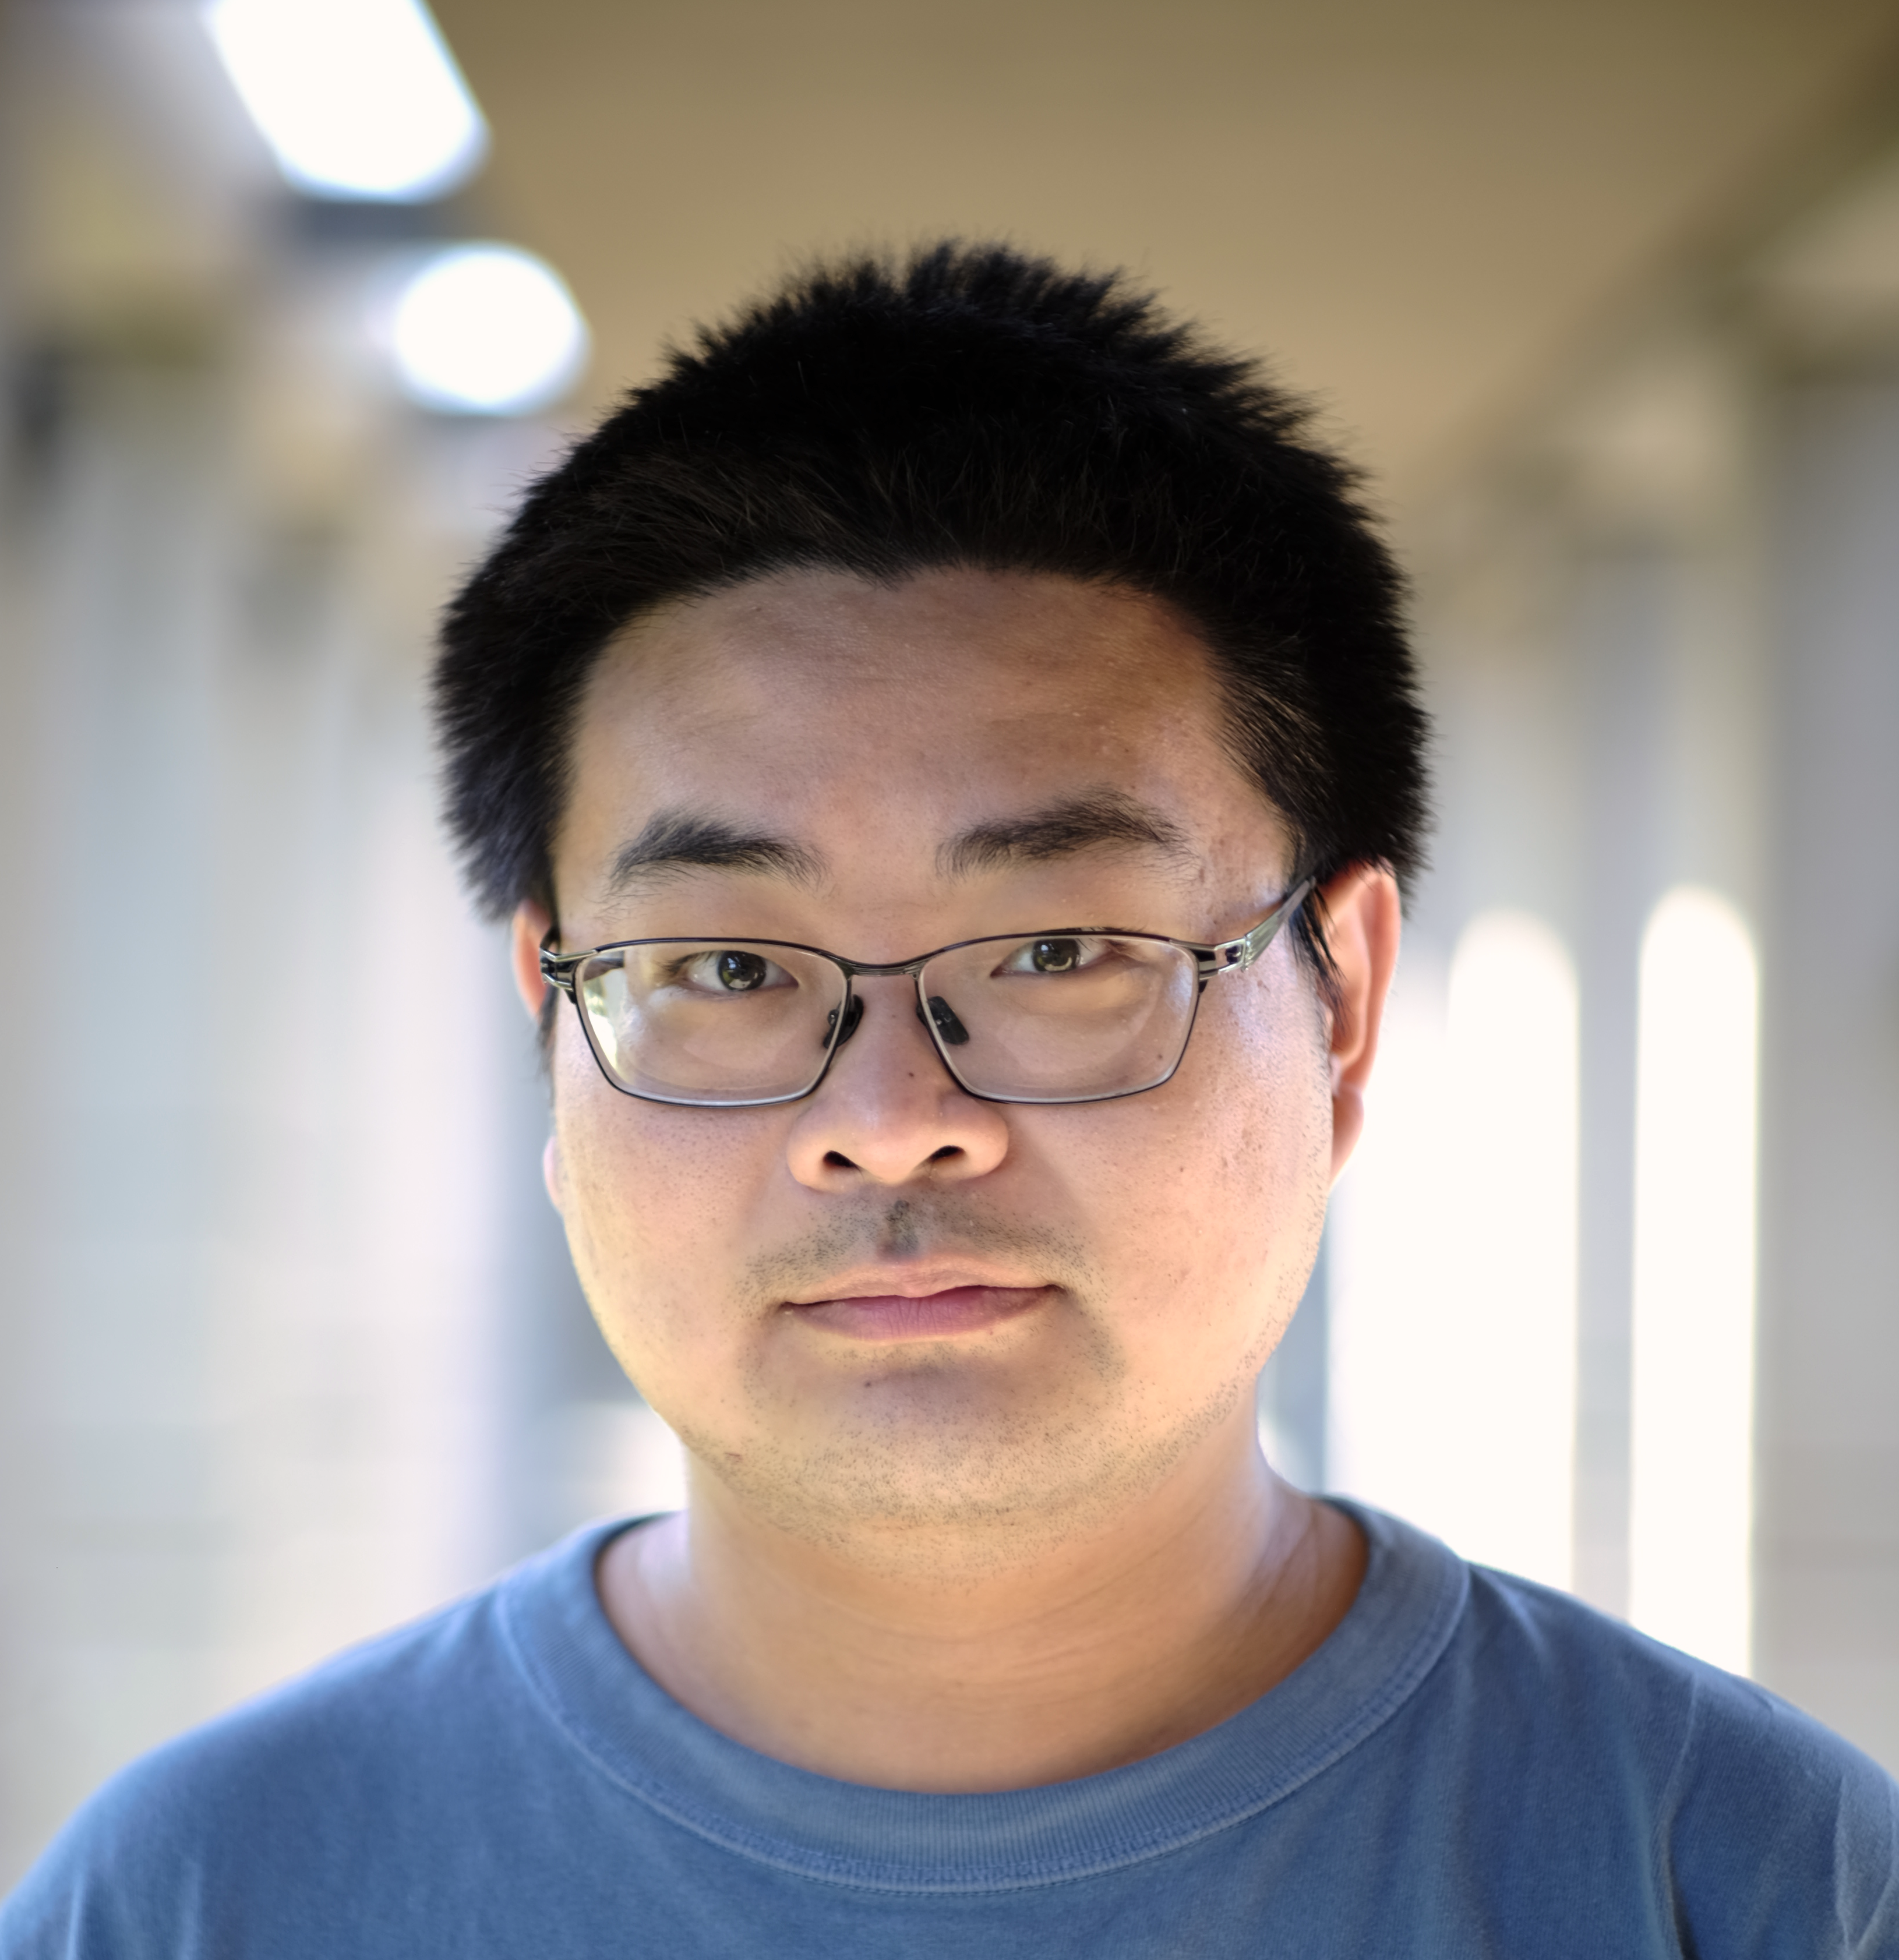
\includegraphics[width=1.1in,height=1.25in,clip,keepaspectratio]{author/chisheng.png}}]{ Chi-Sheng Chen} received a bachelor degree in Electrophysics from National Chiao Tung University and a master's degree in Biomedical Electronics and Bioinformatics from National Taiwan University. He is currently working at a financial AI startup and also serves as an AI project researcher at Harvard Medical School and Beth Israel Deaconess Medical Center. His research expertise includes time-series analysis, computer vision, brain-computer interfaces (BCI), electroencephalography (EEG), multimodal contrastive learning, and quantum machine learning. Chen has led the development of foundational models for EEG-based image generation, aiming to improve psychiatric treatment and the discovery of biomarkers for drug development. He has designed hybrid quantum-classical architectures for EEG encoding and pioneered quantum deep learning methods for contrastive learning between EEG and visual data. His research also focuses on medical speech processing and the integration of multimodal large language models (LLMs) for clinical and financial application.
\end{IEEEbiography}

\begin{IEEEbiography}[{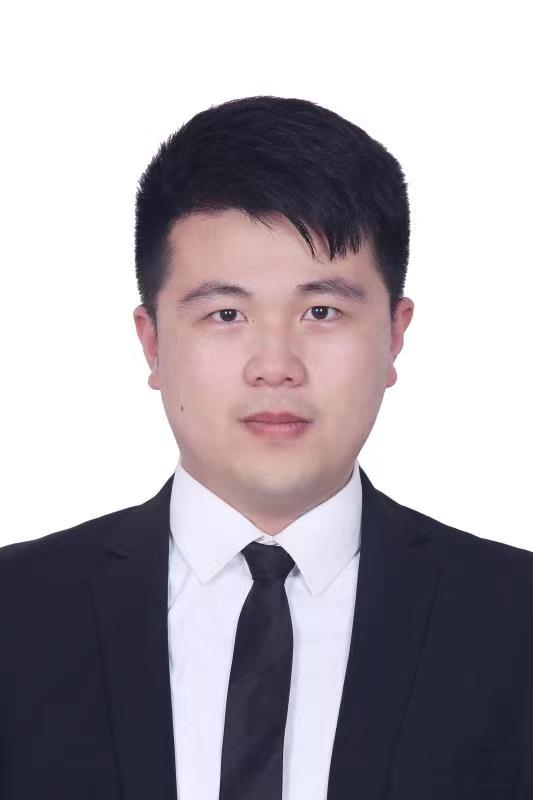
\includegraphics[width=0.9in,height=1.1in,clip,keepaspectratio]{author/Xinyu.jpg}}]{Xinyu Zhang} received the B.E. and the M.S. degree from the Information and Automatic College, Tianjin University of Science and Technology, Tianjin, China, in 2019 and 2022, separately, where he is currently pursuing the Ph.D. degree in intelligent system engineering with Luddy School of Informatics, Computing, and Engineering, Indiana University Bloomington, Bloomington, IN, USA.
His main research includes quantum neural network, deep learning, advanced signal processing, and other disciplines such as information science and large language models (LLMs).
\end{IEEEbiography}


\begin{IEEEbiography}[{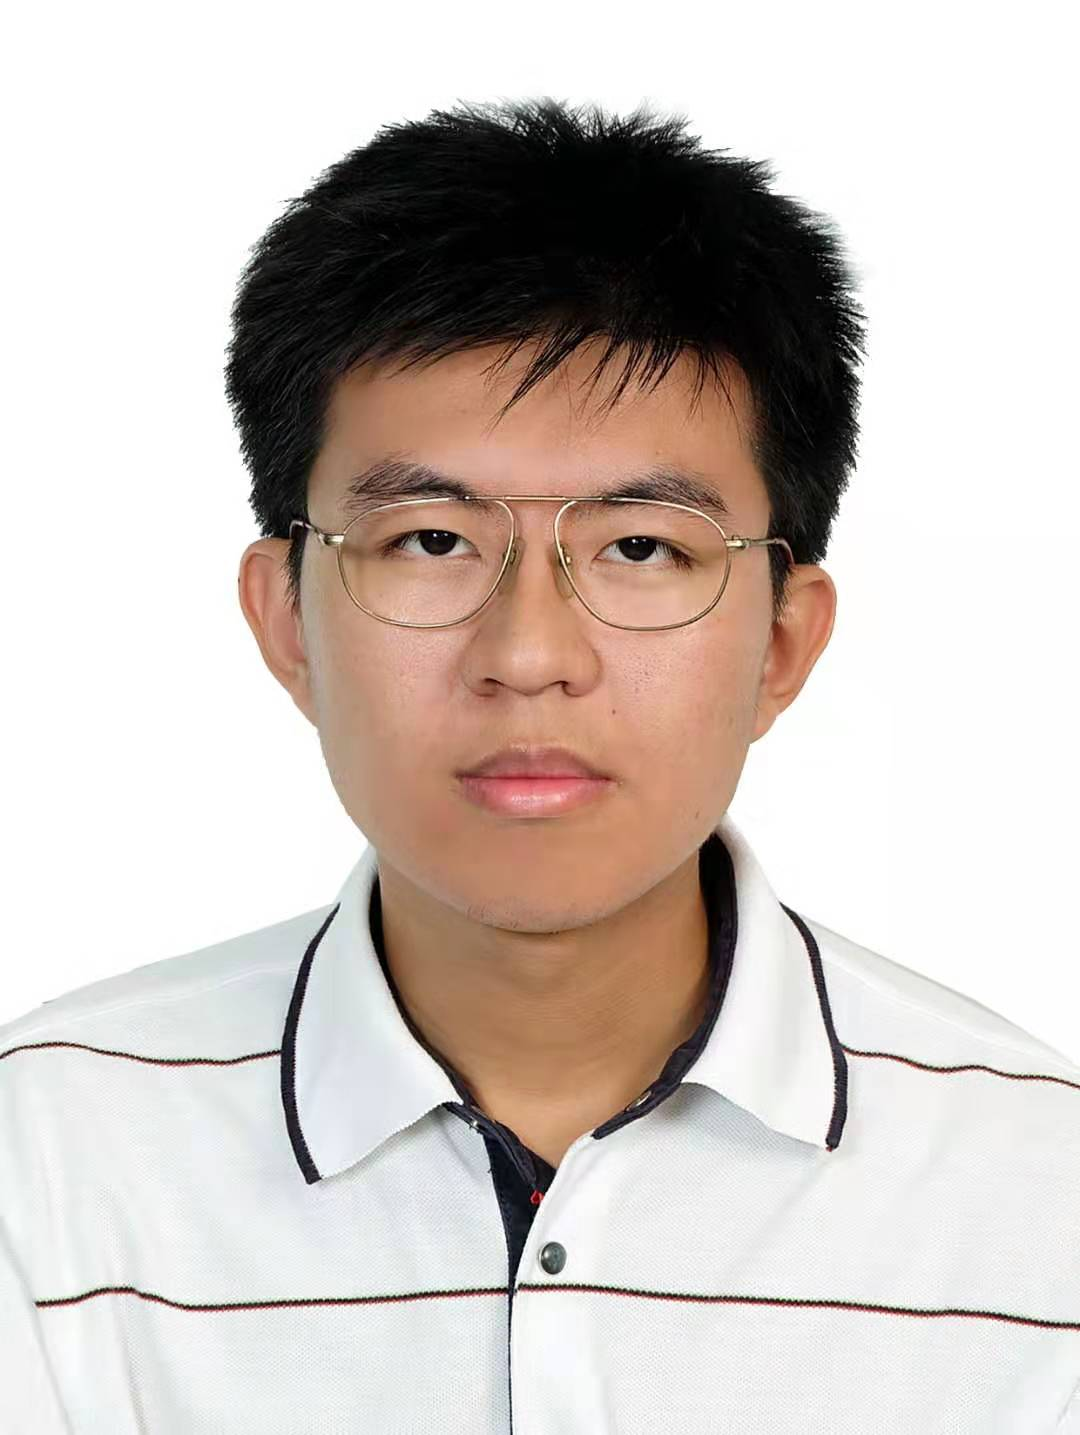
\includegraphics[width=1in,height=1.25in,clip,keepaspectratio]{author/enjui.jpg}}]{En-Jui Kuo}   received the B.S. degree in electrophysics from National Yang Ming University, Taipei, Taiwan. He then obtained his M.S. degree in physics from National Taiwan University, Taipei, Taiwan, and completed his Ph.D. in physics at the University of Maryland, USA. Currently, he is an Assistant Professor of department of electrophysics at the National Yang Ming Chiao Tung University, Taiwan.
\end{IEEEbiography}



\begin{IEEEbiography}[{
\includegraphics[width=0.9in,height=1.1in,clip,keepaspectratio]{author/Rong.jpg}}]{Rong Fu} received the B.S. degree in Communication Engineering from Jiangsu Ocean University, Jiangsu, China, in 2018, and the M.S. degree in Electronic Information Engineering from the College of Information and Automation, Tianjin University of Science and Technology, Tianjin, China, in 2023. She is currently pursuing the Ph.D. degree in Intelligent Systems Engineering with the Luddy School of Informatics, Computing, and Engineering, Indiana University Bloomington, Bloomington, IN, USA. Her research interests include signal processing and deep learning.
\end{IEEEbiography}

\begin{IEEEbiography}[{
\includegraphics[width=0.9in,height=1.1in,clip,keepaspectratio]{author/qiuzhe.jpg}}]{Qiuzhe Xie} received a bachelor's degree in Electrical Engineering from Hefei University of Technology and a master's degree in Electronics Engineering from National Cheng Kung University, followed by a Ph.D. in Electronics Engineering from National Taiwan University. His research expertise encompasses biosensors, advanced semiconductor processes, nanomaterials, and microfabrication techniques. He has spearheaded the development of nano-structural electrode arrays with ultra-thin dielectric stacking and leveraged quantum computing algorithms to enhance sensing precision. Furthermore, he has engineered CRISPR-based electrochemical sensors and developed innovative water purification systems for semiconductor manufacturing. Extending his work to practical application, he also focuses on the commercialization of medical devices, having validated business models for cardiosensor technologies through the NSF program.
\end{IEEEbiography}

\begin{IEEEbiography}[{
\includegraphics[width=0.9in,height=1.1in,clip,keepaspectratio]{author/fan.jpg}}]{Fan Zhang} received the B.S. degree in Statistics from Beijing Normal University, Beijing, China, in 2016, the M.S. degree in statistics from National Cheng Kung University, Taiwan, in 2018, and the Ph.D. degree in statistics from Arizona State University, Tempe, AZ, USA, in 2024. She is currently an Assistant Professor with the Department of Mathematics, Boise State University, Boise, ID, USA. Her research interests include design and analysis of experiments, variable selection, uncertainty quantification, Bayesian modeling and inference, and quantum-enhanced machine learning.

\end{IEEEbiography}


\end{document}
